%Preámbulo del documento

\documentclass[letterpaper]{article} %Tipo de documento
\usepackage[utf8]{inputenc} % Codificación del texto
\usepackage[spanish]{babel} %Idioma del documento
\usepackage{graphicx} %Inserción de imagenes
\usepackage{amssymb, amsmath} %Fórmulas matemáticas
\usepackage{float}
\usepackage[caption = false]{subfig}

%Cuerpo del documento

\begin{document}

    \begin{figure}[H]
        \begin{titlepage}%Cuerpo de la portada
            
            \centering
            \subfloat{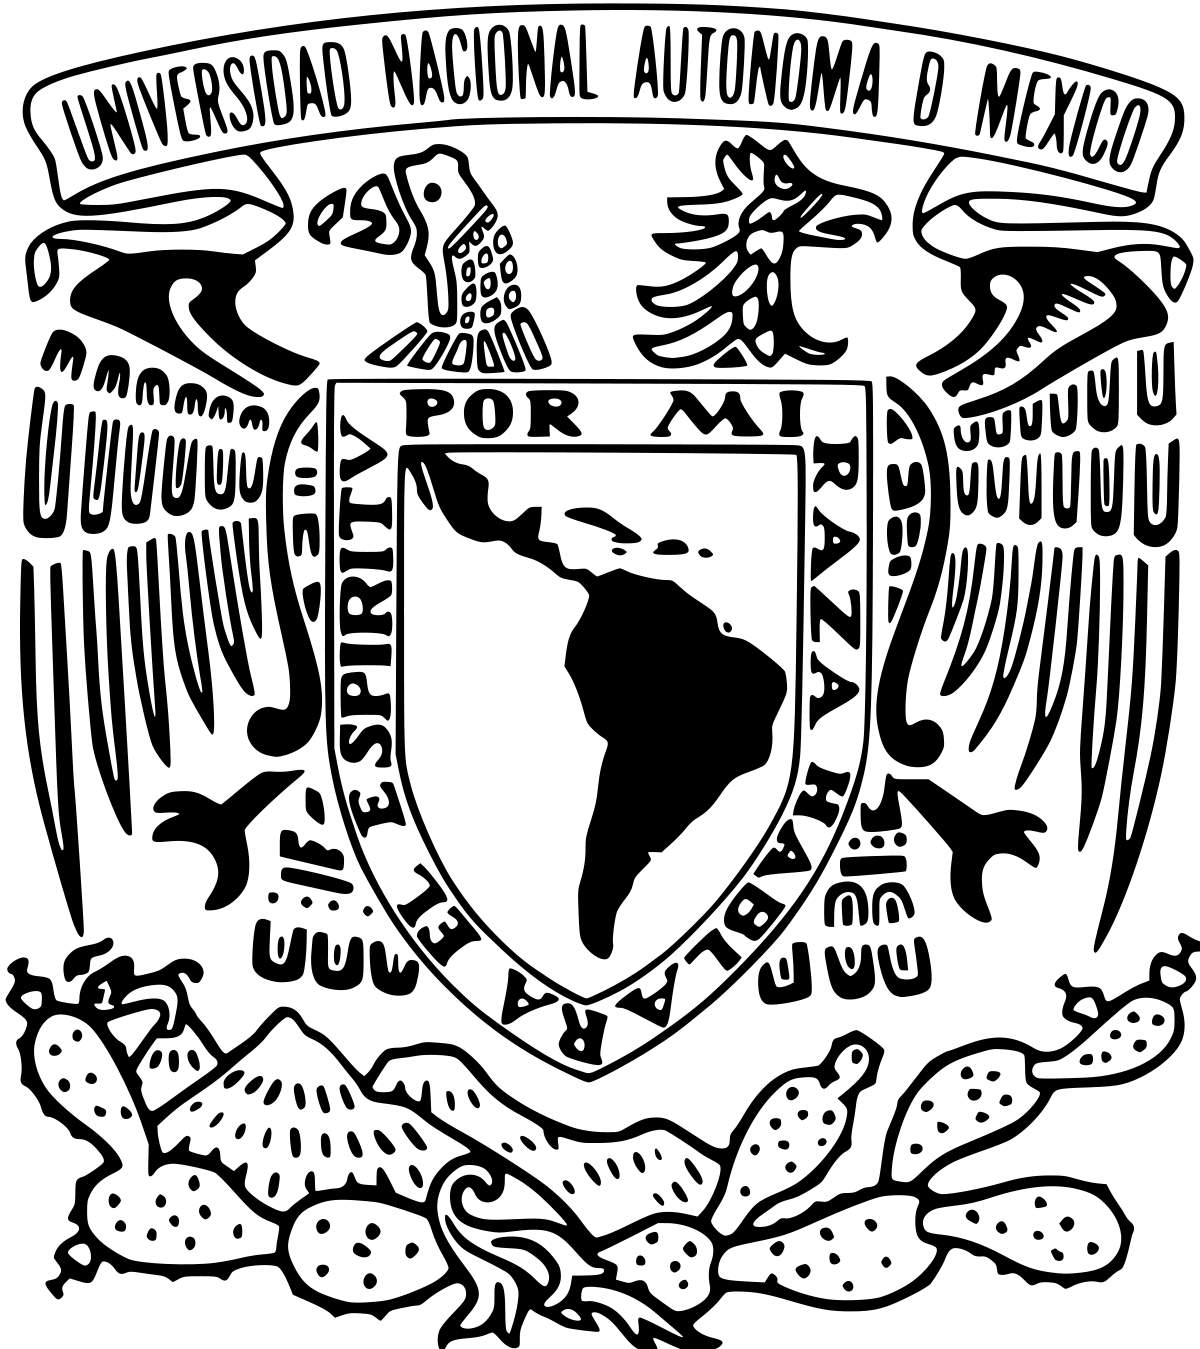
\includegraphics[width=0.2\textwidth]{unamescudo.png}\par}
            \hspace{7cm}
			\subfloat{
\includegraphics[width=0.2\textwidth]{escudofi_negro}\par}

            \vspace{1cm}
                                    
            \centering
            {\bfseries\LARGE Universidad Nacional Aut\'onoma de M\'exico \par}
            \vspace{1cm}
            {\bfseries\LARGE Facultad de Ingenier\'ia \par}
            \vspace{1cm}
            {\bfseries\LARGE Divisi\'on de Ingenier\'ia El\'ectrica\par}
            \vspace{1cm}
            {\itshape\Large \textbf{Laboratorio de Diseño Digital Moderno\\} \par} 
            \vspace{1cm}
            {\scshape\LARGE{Pr\'actica 2: Lenguaje de descripci\'on de hardware VHDL\\} \par}
            \vspace{1cm}
            {\itshape\Large \textbf{M.I Vicente Flores Olvera\\} \par}
            \vspace{1cm}
            \vfill
            {\itshape\Large Bautista P\'erez Brian Jassiel \\\par}
            {\itshape\Large Serralde Flores Andrea \\\par}
            \vfill
            \vspace{1cm}
            {\itshape\Large \today\par}
            
        \end{titlepage}
	\end{figure}
    \newpage

    \section*{1. Objetivo}

    \textbf{El alumno analizar\'a de qu\'e partes esenciales contra un c\'odigo hecho
    a traves del lenguaje de hardware VHDL, as\'i tambi\'en que implica la implemenaci\'on
    de funciones mediante el estilo de flujo de datos.}


    \section*{2. Previo}

    Obtener las formas m\'inimas SOP y POS al igual que las formas can\'onicas de las funciones del
    combinacional representado por un sistema que tiene cuatro entradas \textbf{A; B; C; D} y 
    cuatro salidas, \textbf{W; X; Y; Z}. La salida representa un n\'umero en c\'odigo Exceso - 3 cuyo
    valor es igual al n\'umero de unos presentes en la entrada. Por ejemplo, si
    ABCD = 1101, entonces la salida debe ser WXYZ = 0110.

    \vspace{0.5cm}

    \textbf{Obtenci\'on de las funciones mediante tablas de verdad}

    \vspace{0.5cm}

    \begin{table}[H]
        \begin{center}
            \begin{tabular}{| c | c |}
                \hline
                ABCD & xyz \\ \hline
                0000 & 011 \\
                0001 & 100 \\
                0010 & 100 \\
                0011 & 101 \\
                0100 & 100 \\
                0101 & 101 \\
                0110 & 101 \\
                0111 & 110 \\
                1000 & 100 \\
                1001 & 101 \\
                1010 & 101 \\
                1011 & 110 \\
                1100 & 101 \\
                1101 & 110 \\
                1110 & 110 \\
                1111 & 111 \\ \hline
                \end{tabular}
                \caption{Tabla de verdad de las funciones.}
                \label{tab:verdad}
            \end{center}
    \end{table}

    \textbf{Finalmente, las funciones nos quedan de la siguiente forma:}
    \vspace{0.5cm}


        $x = a + b + c + d$

        \vspace{0.5cm}

        $y  = ab(d + c) + cd(b + a) + \overline{a}\overline{b}\overline{c}\overline{d}$
    
        \vspace{0.5cm}

        $z = \overline{a \oplus b \oplus c \oplus d}$
        
        \vspace{0.5cm}

    \begin{itemize}
        \item ¿Qu\'e son las bibliotecas, la entidad y la arquitecura en una estructura desrita en VHDL?\\
            R. Las \textbf{bibliotecas}, dentro de VHDL, son colecciones de piezas de código usualmente empleadas.
            Esto permite poder reusar esas piezas o compartirlas con otros diseños.\\
            La \textbf{entidad} Es la zona de declaraci\'on de los vectores del m\'odulo, generalmente 
            entradas y salidas \\
            La \textbf{arquitectura} Es la zona en la cual se describe de manera detallada la estructura interna
            o comportamiento del m\'odulo.
        \item Investiga c\'omo se realiza la asignaci\'on de una funci\'on o de un valor en VHDL. \\
            R. La asignaci\'on de funciones se realiza mediante el operador $<=$. A la izquierda se escribe el nombre o identificador
            de la funci\'on o variable, mientras que a la derecha se escribe lo que se le va a asignar.
        \item ¿Qu\'e significa el t\'ermino concurrente dentro del lenguaje VHDL? \\
            R. Es la implementaci\'on de procesos dentro de un archivo de programaci\'on VHDL. Su prop\'osito es definir
            los l\'imites de un dominio secuencial.
    \end{itemize}


    \section*{3. Desarrollo de la pr\'actica}
        \subsection*{3.1. Pr\'actica 2A}
        Programar las funciones mostradas, en un formato SOP y POS m\'inimo (reducido) en
        forma de flujo de datos, para su posterior simulaci\'on dentro de la plataforma Quartus II.

        \begin{equation}
            \label{eq:POS}
            f(xyzt) = (x + \bar{x}y + \overline{yt})(x + (\overline{xy})z)
        \end{equation}

        Funci\'on con formato de Producto de Sumas~\ref{eq:POS}.

        \begin{equation}
            \label{eq:red1}
            f(xyzt) = (x + z)
        \end{equation}

        Funci\'on reducida~\ref{eq:red1}.

        \begin{equation}
            \label{eq:SOP}
            f(uvtw) = vt(u + t\bar{w})(u + \bar{w}) + wu(v +t)
        \end{equation}

        Funci\'on con formato de Suma de Productos~\ref{eq:SOP}.

        \begin{equation}
            \label{eq:red2}
            f(uvtw) = vtu + vt\bar{w} + wut +wuv
        \end{equation}

        Funci\'on reducida~\ref{eq:red2}.

            \subsubsection*{3.1.1. Implementaci\'on en Quartus II}

                \begin{figure}[H]
                    \raggedright
                    \subfloat[Implementaci\'on de las funciones en Quartus II]{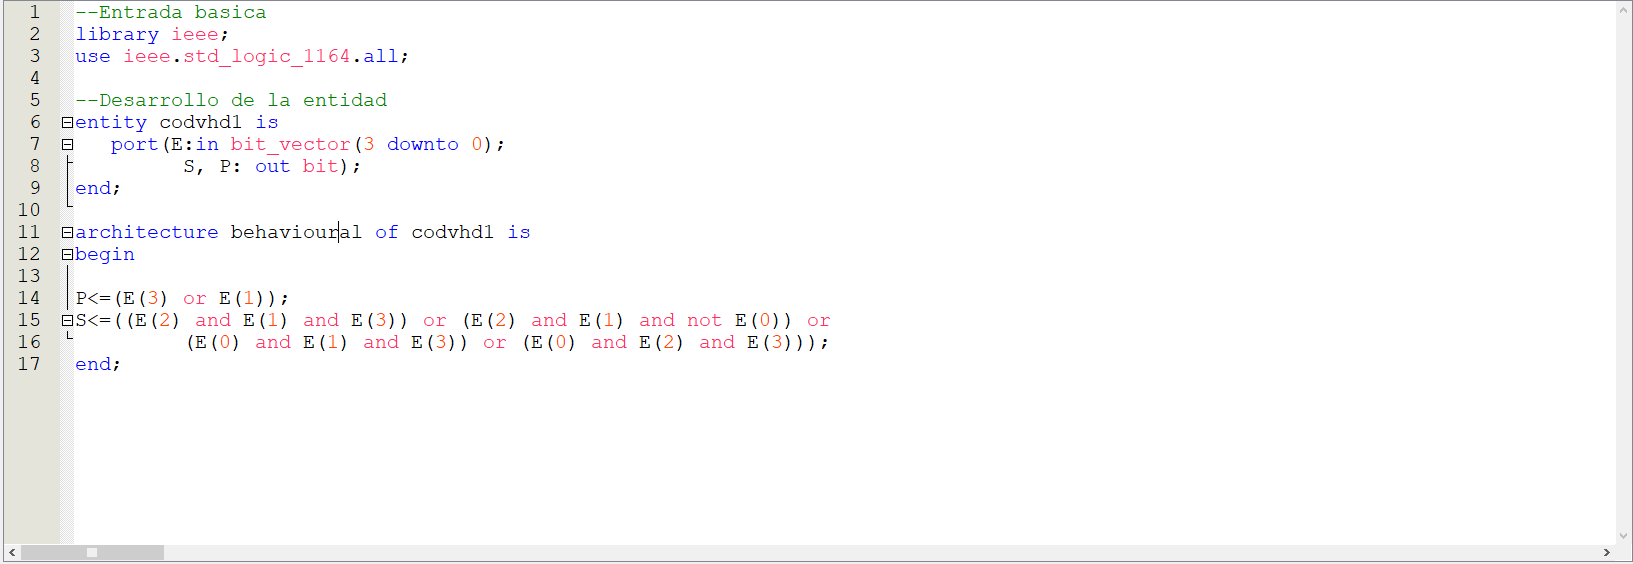
\includegraphics[width = \textwidth]{Codigo1.PNG}}
                \end{figure}

                En este c\'odigo VHDL se importa la biblioteca \textbf{ieee}, despu\'es, dentro de una 
                entidad procedemos a declarar un vector \textbf{E}, el cual va a representar nuestras variables de entrada
                en donde el bit m\'as significativo en cada funci\'on ser\'a \textbf{x} y \textbf{u}, respectivamente.
                Dentro de esta entidad, declaramos nuestras variables de salida, las cuales ser\'an nuestras funciones y representadas
                en SOP y POS, dichas funciones est\'an representadas por las variables \textbf{P} y \textbf{S}, respectivamente. 
                Finalmente, dentro de una arquitectura procederemos a declarar nuestras funciones, en las cuales, debemos de ser muy 
                cuidadosos con la jerarqu\'ia y con los par\'entesis para que no tengamos errores durante la compilaci\'on de nuestro proyecto.

                \begin{figure}[H]
                    \raggedright
                    \subfloat[Esquema de las funciones]{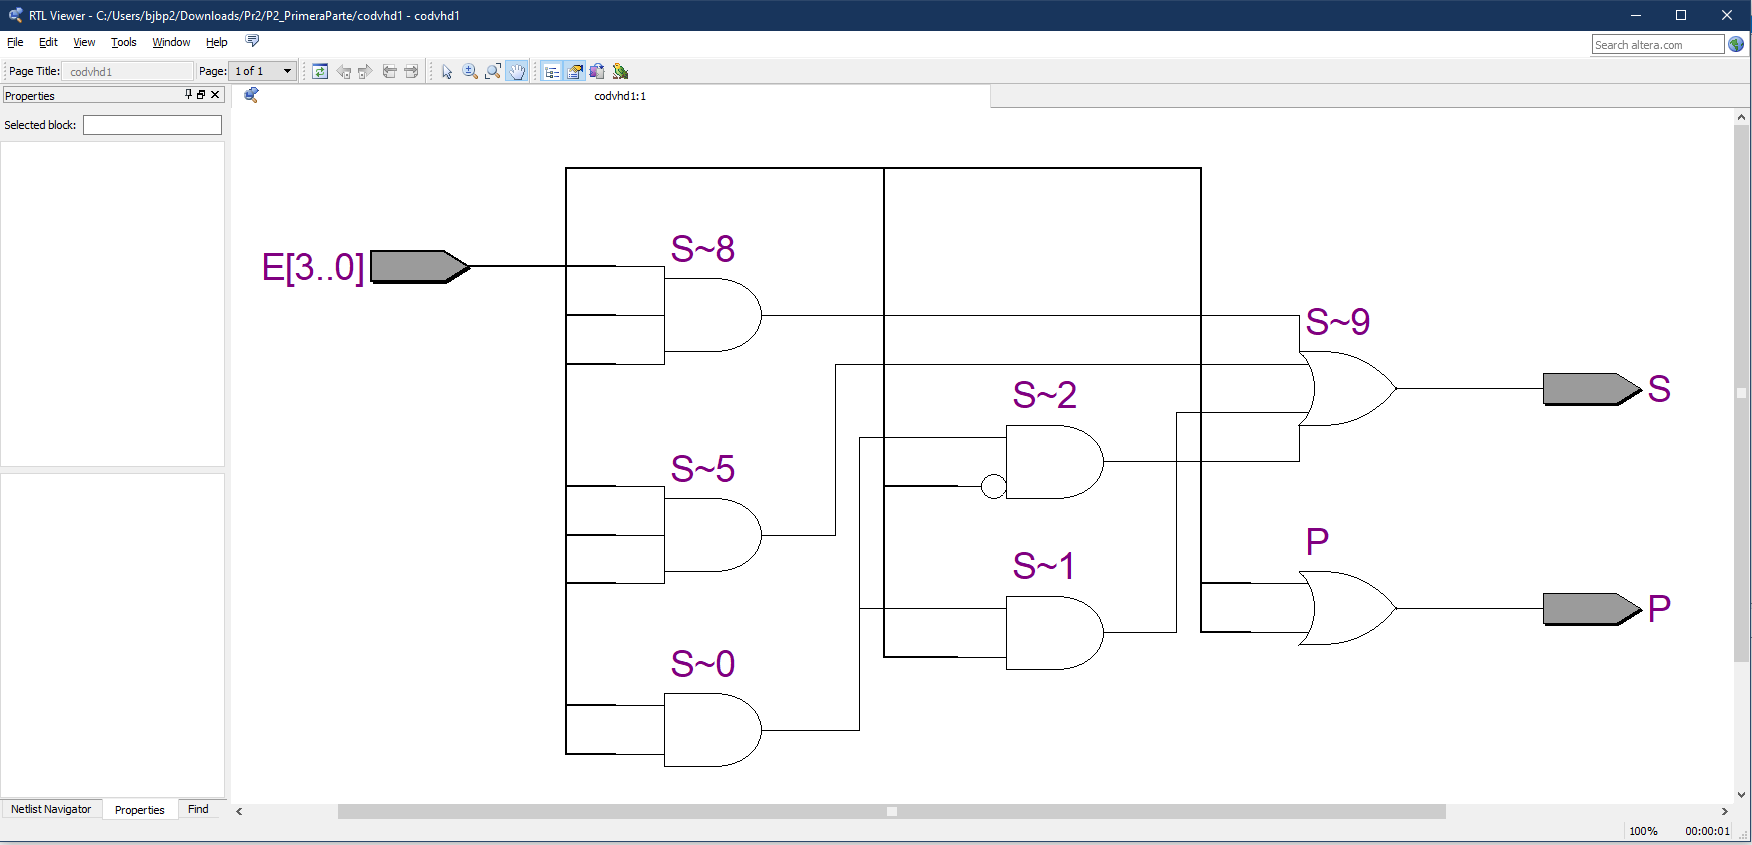
\includegraphics[width = \textwidth]{RTLVPT1.PNG}}
                \end{figure}

                En el esquema de arriba se representa el c\'odigo reci\'en escrito en forma de un
                circuito l\'ogico, en este caso vemos que dicho circuito est\'a compuesto de compuertas
                \textbf{and} y \textbf{or}

                \begin{figure}[H]
                    \raggedright
                    \subfloat[Simulaci\'on realizada]{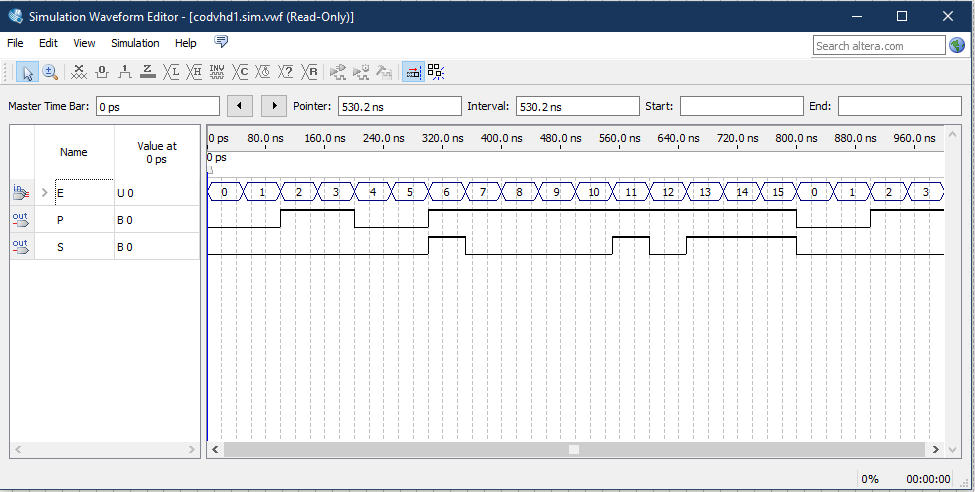
\includegraphics[width = \textwidth]{SimulacionPT1.PNG}}
                \end{figure}

        \subsection*{3.2. Pr\'actica 2B}
        Programar las funciones expresadas en formato POS Y SOP can\'onicas y m\'inimas del previo
        en forma de flujo de datos, para su posterior simulación dentro de la plataforma Quartus II.

        \subsubsection*{3.2.1. Implementaci\'on en Quartus II}

            \begin{figure}[H]
                \raggedright
                \subfloat[Implementaci\'on de las funciones en Quartus II]{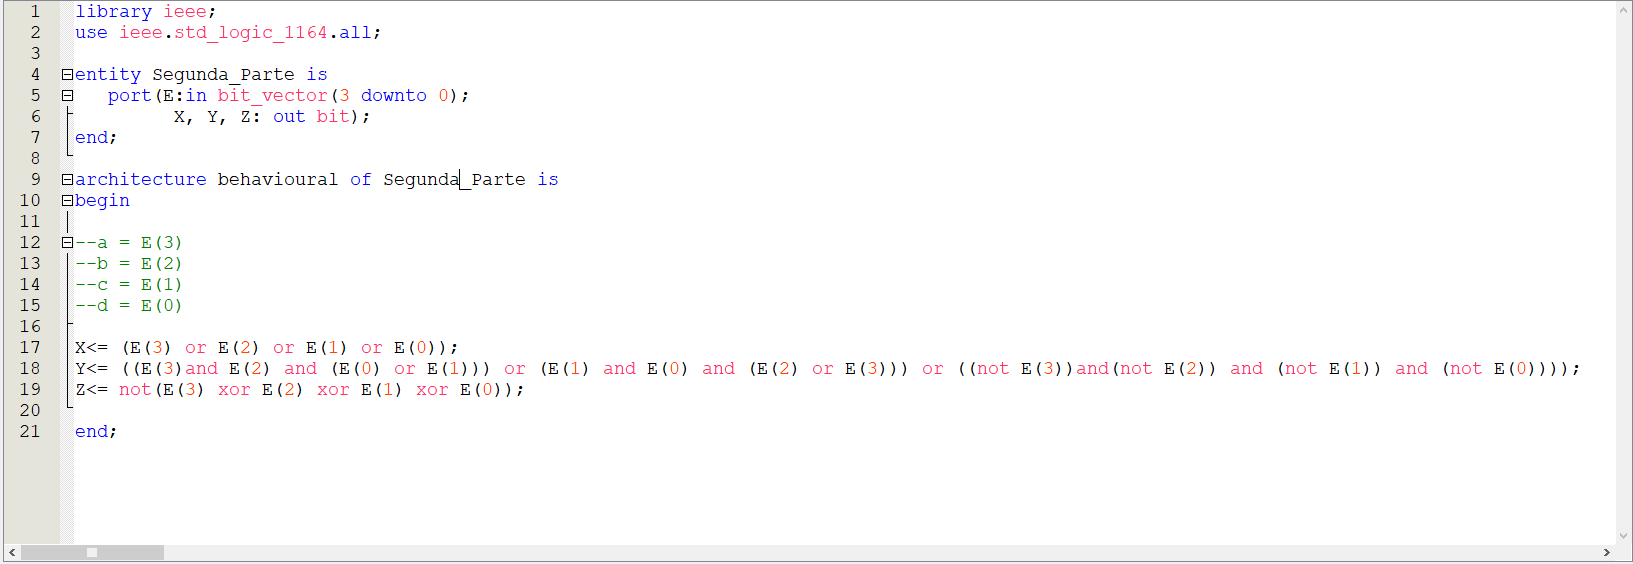
\includegraphics[width = \textwidth]{Codigo2.PNG}}
            \end{figure}

            Esta implementaci\'on tiene una forma similar, que al primer ejercicio realizado, la diferencia est\'a 
            en que declaramos tres variables de salida, \textbf{x, y, z} en la arquitectura en donde declaramos nuestras funciones.
            El proceso de compilaci\'on y ejecuci\'on del programa es el mismo. 

            \begin{figure}[H]
                \raggedright
                \subfloat[Esquema de las funciones]{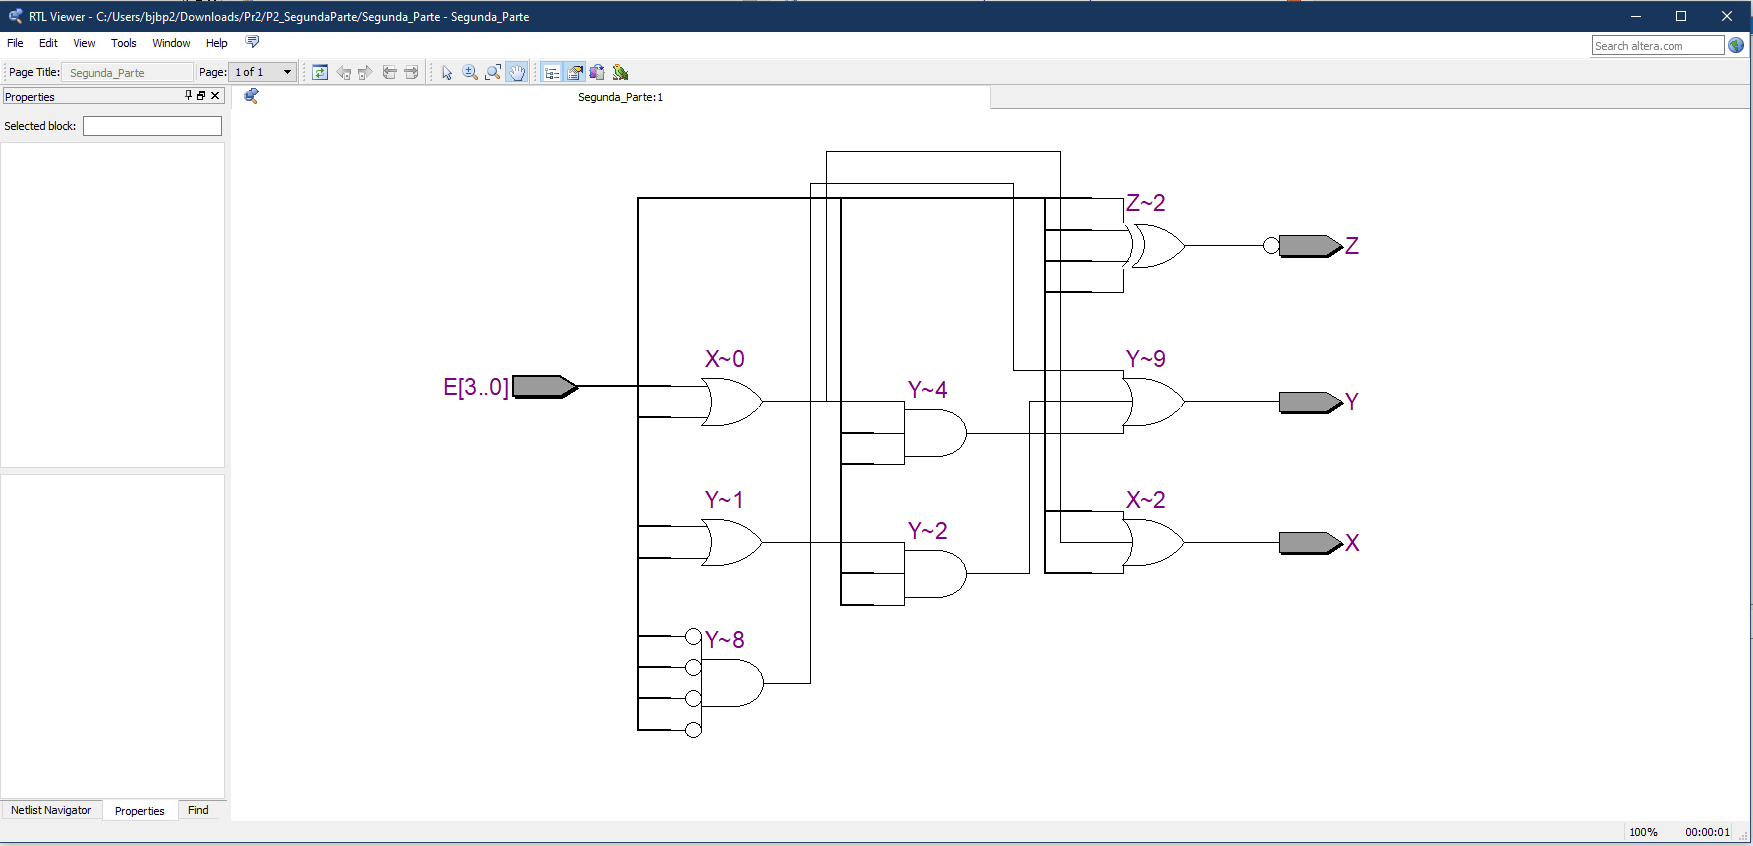
\includegraphics[width = \textwidth]{RTLVPT2.PNG}}
            \end{figure}

            En este diagrama se ve representado nuestro c\'odigo en un circuito l\'ogico compuesto por compuertas
            \textbf{and, or} y \textbf{xor}.             

            \begin{figure}[H]
                \raggedright
                \subfloat[Simulaci\'on realizada]{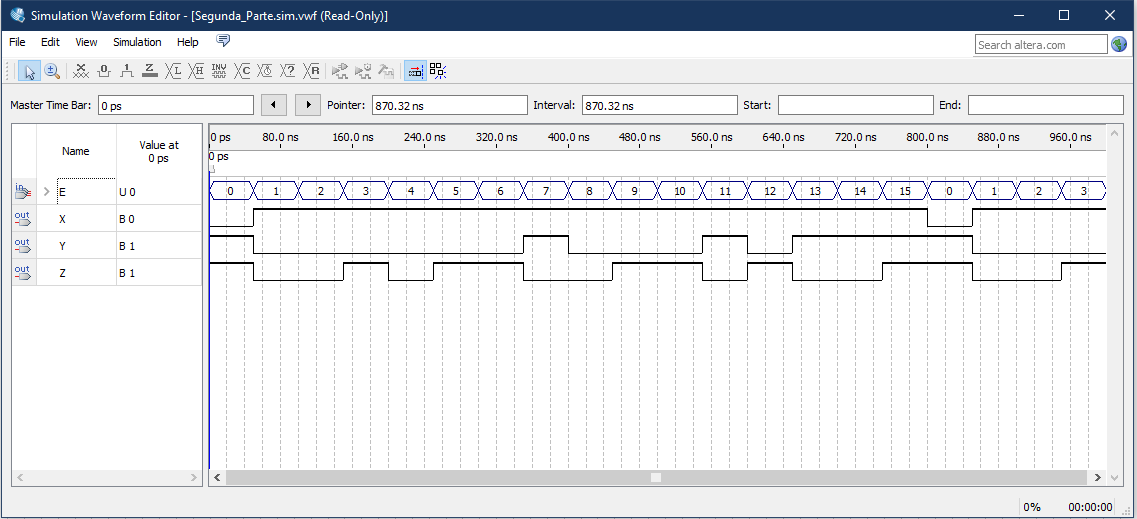
\includegraphics[width = \textwidth]{SimulacionPT2.PNG}}
            \end{figure}

            En esta simulaci\'on verificamos que la tabla de verdad realizada para obtener las funciones es
            igual a la que obtuvimos en Quartus, por lo que se deduce que realizarmos la obtenci\'on y 
            codificaci\'on de las variables de manera correcta.

    \section*{4. Conclusiones}

    Mediante la aplicac\'on de las leyes del \'algebra de Boole se pudo obtener en primer lugar la representaci\'on can\'onica
    de las funciones y en segundo, las formas reducidas en POS y SOP. Esto nos fue de gran ayuda ya que de m\'as sencillo
    escribirlas en c\'odigo VHDL en el simulador Quartus II. 

    Al observar que los resultados de la simulación coinciden con las tablas de verdad realizadas para la representaci\'on de las funciones
    se concluye que el objetivo principal de esta pr\'actica se cumpli\'o de manera satisfactoria.  \\
    El lenguaje VHDL fue muy importante para la realizaci\'on de esta pr\'actica y ser\'a una herramienta muy \'util para las pr\'oximas y tambi\'en
    para el desarrollo de programas para las tarjetas programables, no s\'olo en esta materia, sino en las de los siguientes semestres.

\end{document}